\documentclass[../Book.Stress_regulation.tex]{subfiles}
\graphicspath{{\subfix{../images/}}}
\begin{document}

\label{Ex:SunSalutation}
\begin{figure}[htb!]
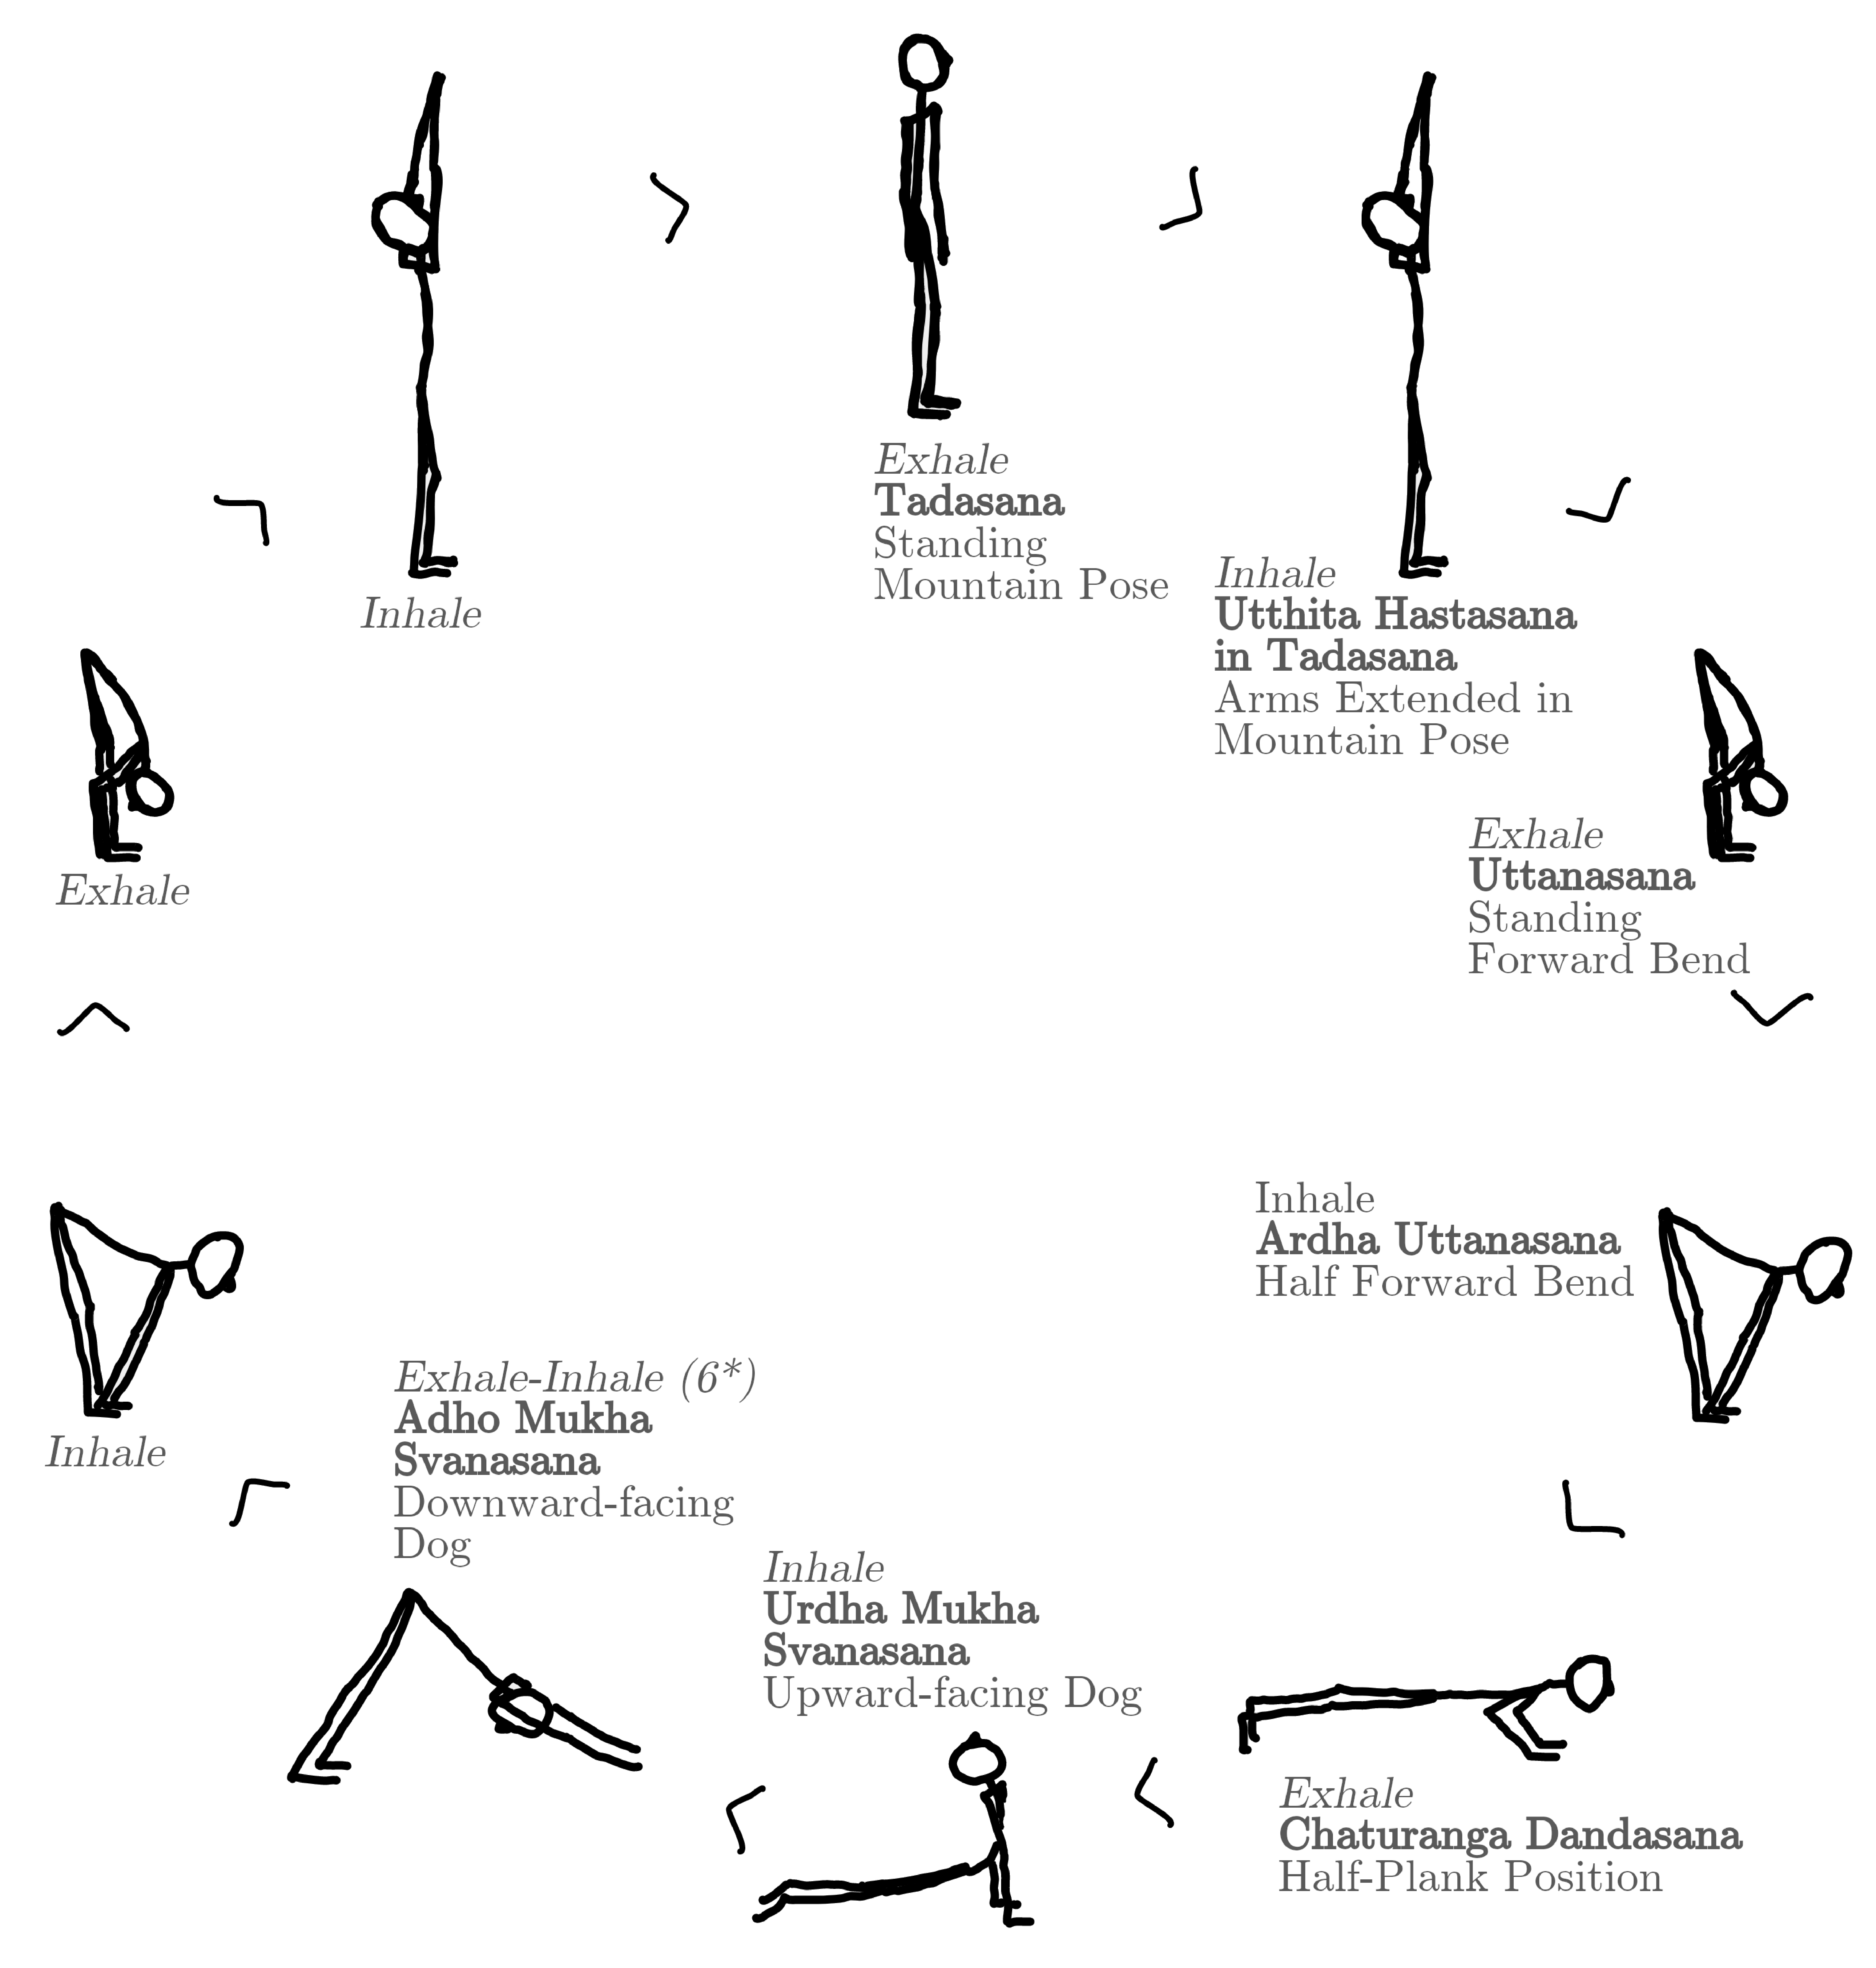
\includegraphics[width=13cm]{SunSalute}\label{sf:yoga}
\caption{Sun salutation --- Surya Namaskar}
\end{figure}

%------------------------------------------------------------
%------------------------------------------------------------

The Sun Salutation\index{sun salutation} (sanskrit: Surya Namaskar) increases your physical strength, flexibility, your inner balance and your mental clarity.
Practiced first thing in the morning, it gets you instantaneously awake and active.
Practiced in the evening, it helps free up blocked energies.

The sun salutation is classical exercise from yoga, which consist in a fluid motion which goes through multiple positions.
The Sun Salutation stimulates all internal organs, stretches and twists the spinal cord, all the limbs and all muscle groups.
If you practice ti on a regular base you will notice how it gives you strength and how you will get flooded with energy.

\begin{itemize}
\item Your breath determines the speed.
  Upon inhalation, the spine gets stretched backwards, on exhale it gets stretched forward.
  Breather calmly while executing this exercise, but consciously.
\item Make sure that you practice it in fresh air.
  Make sure that your body can move freely (no tight clothes, bare foot).
  The sun salutation is best practices before meals, otherwise your energy and your blood are going to be occupied with digestion.
\item Execute all exercises calmly and without pressure. If you are not flexible enough yet for a posture, then go as far as you are able to go, without forcing it.
  It's important that the movements are executed fluidly and consciously --- in your mind intended as a salutation to the sun.
\item In the beginning, you will probably be unable to bring your head down to your knees, or touching the ground with your palms while bending forwards.
  Keep your patience and your sense of fun. In the beginning it's enough if the tip of your fingers touch the ground.
  Your body has to first get used to the movements and with these exercises it will get more flexible and will get to move smoothly.
\end{itemize}

\subsubsection{1. Mountain Pose: Stand upright}
\begin{enumerate}
\item Put your feet with frim pressure on the ground. Pay attention that your toes don't claw into the ground.
\item Stretch your knees. By doing this, your legs will get stretched (exception: people with knee problems: leave your knees slightly bend).
\item Turn the tailbone down and forward, tense up the muscles of the pelvic floor and the sphincter of your anus. The pelvis lifts up.
\item Tense up the abs.
\item Widen and lift your chest.
\item Bend your shoulder blades backwards and lower them.
\item Feel into the posture, from the feet up the the crown.
\item Put your hands into a salutation pose and focus on the area of your heart.
\item Slightly lower your head.
\item Let your breath flow slowly and calmly.
  \item Interlock your thumbs and exhale deeply.
  \end{enumerate}

\end{document}